\documentclass[12pt,letterpaper]{book}
\usepackage[utf8]{inputenc}
\usepackage[english]{babel}
\usepackage{amsmath}
\usepackage{amsfonts}
\usepackage{amssymb}
\usepackage{makeidx}
\usepackage{graphicx}

\usepackage[left=2cm,right=2cm,top=2cm,bottom=2cm]{geometry}


%My packages

\usepackage{multicol}
\usepackage{colortbl}
\usepackage{mathrsfs}
\usepackage{cite}
\usepackage{float}

\usepackage{hyperref}
\hypersetup{
    colorlinks=true,
    linkcolor=blue,
    filecolor=magenta,      
    urlcolor=cyan,
}

\urlstyle{same}




\newtheorem{definition}{Definition}
\newtheorem{theorem}{Theorem}[section]
\newtheorem{corollary}{Corollary}[theorem]
\newtheorem{lemma}[theorem]{Lemma}
\newtheorem{example}{Example}[section]
\newtheorem{exercise}{Ejercicio}[section]
\newtheorem{question}{Pregunta}[section]
\newtheorem{sabias}{¿Sabias que...?}[section]

\title{Notes of Electromagnetic Fields}



\author{Esteban}
\begin{document}
\maketitle
\tableofcontents


\chapter{Maxwell's equations}



\begin{table}[H]
        \caption{}
        \label{DSA}
        \begin{center}
        \begin{tabular}{|p{5cm}||p{5cm}||p{5cm}|}
        \hline        
         & Integral form&Differential form \\ \hline
         \tiny{Gauss's law} &   &    \\ \hline
         \tiny{Magnetic field of the magnetic flux}&  &  \\ \hline
        \end{tabular}
        \end{center}
    \end{table}
    \vspace{0.2 cm}



\chapter{Transformation Coordinates}

Assume that you have the follow joint of fields whose  functions are in different coordenate systems

\begin{equation*}
\begin{aligned}
F=f(x)a_x+f(y)a_y+f(z)a_z\\
F=f({\rho })a_{\rho }+f({\phi })a_{\phi }+f(z)a_z\\
F=f({r })a_{r}+f({\theta })a_{\theta }+f({\phi })a_{\phi }
\end{aligned}
\end{equation*}

Now, How I can do for to change between the different systems? You can review all the time the tables for change of a system to other, but in the university that is not the sense. For that, is better use the follow method that is described by the Equation \eqref{cooTra}.\\


\begin{multline}
\label{cooTra}
\footnotesize{\left[\begin{array}{c}
F=f(x)a_x+f(y)a_y+f(z)a_z\\
F=f({\rho })a_{\rho }+f({\phi })a_{\phi }+f(z)a_z\\
F=f({r })a_{r}+f({\theta })a_{\theta }+f({\phi })a_{\phi }
\end{array}\right]
\left[\begin{array}{ccccccc}
\cdot a_x &\cdot a_y&\cdots &\cdot a_{\rho }&\cdots &\cdot a_r &\cdots \\
\cdot a_x &\cdot a_y&\cdots &\cdot a_{\rho }&\cdots &\cdot a_r &\cdots \\
\cdot a_x &\cdot a_y&\cdots &\cdot a_{\rho }&\cdots &\cdot a_r &\cdots 
\end{array}\right]=}\\
\footnotesize{ \left[\begin{array}{lclclc}
\text{In cartesian system, component x } & &\text{In cilindrical system, component }\phi &  \\
F=f(x)														&	\cdots &F=A_2f(x)+B_2f(y) +C_2f(z)				&\cdots  \\
F=A_1f(\rho )+B_1f(\phi )+C_1f(z) 	&\cdots &F=f(\rho )												&\cdots \\
F=D_1f(r)+E_1f(\theta )+F_1f(\phi ) 	&\cdots &F=D_2f(r)+E_2f(\theta )+F_2f(\phi )  &\cdots  
\end{array}\right.}\\
\footnotesize{ \left.\begin{array}{lclclc}
\text{In spherical system,component r}& \\
F=A_3f(x)+B_3f(y) +C_3f(z)		&\cdots \\
F=D_3f(\rho )+E_3f(\phi )+F_3f(z) &\cdots \\
F=f(\rho )											&\cdots 
\end{array}\right]}
\end{multline}

\textcolor{red}{Important}: If for example I need change from cylindrical coordinates to cartesian coordenates all the variables have that be how the last system. The constants $A_i,B_i,C_i,D_i,E_i,F_i$ are find according to the Figures \ref{carCyl} and \ref{cylSph} \\

To find what are the relation between the different vectors the Figure \ref{carCyl} and \ref{cylSph} are useful

\begin{multicols}{2}  

\begin{figure}[H]
\centering
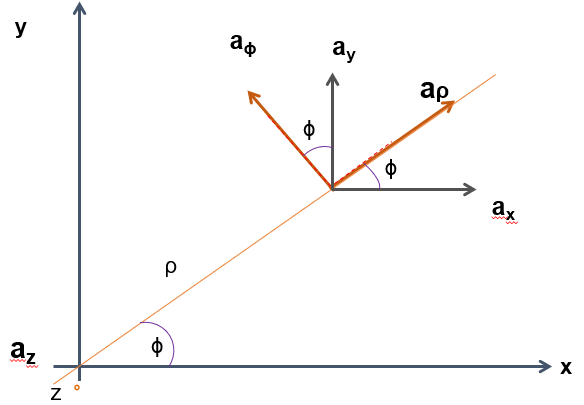
\includegraphics[width=0.7\linewidth]{figures/carCyl.png}
\caption{Relationship between cartesian and cylindrical coordinates \cite{Herrera}}
\label{carCyl}
\end{figure}



\begin{figure}[H]
\centering
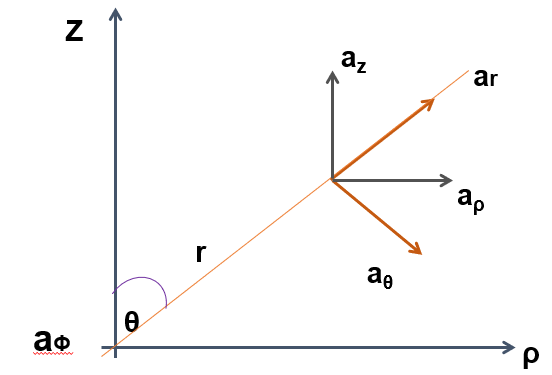
\includegraphics[width=0.7\linewidth]{figures/cylSph.png}
\caption{Relationship between cylindrical and spherical coordinates\cite{Herrera}}
\label{cylSph}
\end{figure}

\end{multicols}

\begin{example}
\begin{multicols}{2}

Find the matrix that change from cartesian coordinates to spherical coordinates and vice versa.\\
 Using the Equation \eqref{cooTra} we have:
\begin{align*}
F\cdot a_x&=f(x)a_x \cdot a_x +f(y)a_y\cdot a_x +f(z)a_z \cdot a_x\\
F\cdot a_x&=f({\rho })a_{\rho } \cdot a_x+f({\phi })a_{\phi }\cdot a_x+f(z)a_z \cdot a_x
\end{align*}


Thus, we obtain:
\begin{align*}
F\cdot a_x&=f(x)\\
F\cdot a_x&=f({\rho })cos(\phi )+f({\phi })cos\left(\phi +\frac{\pi }{2}\right)+f(z)0 \rightarrow\\
f(x)&=f({\rho })cos(\phi )+f({\phi })cos\left(\phi +\frac{\pi }{2}\right)+f(z)0
\end{align*}



Then, the component $y$ es find how,


\begin{align*}
F\cdot a_x&=f(x)a_x \cdot a_y +f(y)a_y\cdot a_y +f(z)a_z \cdot a_y\\
F\cdot a_x&=f({\rho })a_{\rho } \cdot a_y+f({\phi })a_{\phi }\cdot a_y+f(z)a_z \cdot a_y
\end{align*}


Thus, we obtain:


\begin{align*}
F\cdot a_x&=f(y)\\
F\cdot a_x&=f({\rho })cos\left(\frac{\pi }{2}-\phi \right)+f({\phi })cos\left(\phi )\right)+f(z)0 \rightarrow\\
f(y)&=f({\rho })cos\left(\frac{\pi }{2}-\phi \right)+f({\phi })cos\left(\phi )\right)+f(z)0 
\end{align*}


In matrix system we have:\\

$
\left[\begin{array}{c}
f(x)\\
f(y)\\
f(z)
\end{array}\right]
=
\left[\begin{array}{ccc}
cos(\phi )	&	cos\left(\phi +\frac{\pi }{2}\right)	&	0\\
cos\left(\frac{\pi }{2}-\phi \right)	&	cos\left(\phi )\right)	&	0\\
0 & 0 & 1
\end{array}\right]
\left[\begin{array}{c}
f(\rho )\\
f(\phi )\\
f(z)
\end{array}\right]
$\\

Now when a similar development we have:\\
$
\left[\begin{array}{c}
f(\rho )\\
f(\phi )\\
f(z)
\end{array}\right]
=
\left[\begin{array}{ccc}
cos(\phi )	&	cos\left(\phi -\frac{\pi }{2}\right)	&	0\\
cos\left(\frac{\pi }{2}+\phi \right)	&	cos\left(\phi )\right)	&	0\\
0 & 0 & 1
\end{array}\right]
\left[\begin{array}{c}
f(x)\\
f(y)\\
f(z)
\end{array}\right]
$\\

\end{multicols}

\end{example}


\chapter{Space Charge Distribution}

There are four ways of represent the Space Charge Distribution the Figure \ref{chargeDistribution}. All the quantities are scalars if for example were vectors will be electric flux density.   

\begin{figure}[H]
\centering
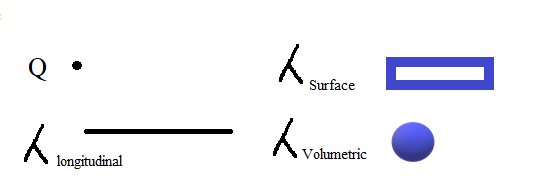
\includegraphics[width=.5\linewidth]{figures/chargeDistribution.png}
\caption{Space Charge Distribution}
\label{chargeDistribution}
\end{figure}

This are some observations
\begin{itemize}
\item Point load: When we do a comparison with other thing and we determinate that is despicable.
\item $\lambda _{longitudinal}$: when in a bar the diameter in very small with respect to the length.
\item $\lambda _{surfaces}$ : the thickness is despicable with respect to total area.
\item $\lambda _{Volumetric}$: All the physical dimensions are important.
\end{itemize}

Now the questions to answers is : How is the electric field E and D?\\

\large{Coulomb's  Law }

\begin{equation}
F=\frac{kQ_0 q}{R^2}a_r\; [N]
\end{equation}
Where $k=\frac{1}{4\pi \epsilon _0}\left[\frac{m^2N}{C^2}\right] $

Its means is:

\begin{itemize}
\item F is directly proportional to the product between the source and the prove charge.
\item The net force appears in the action line.
\item The signs determine if the strength is of attraction or repulsion.
\item The electric force is inversely proportional to the square of the distance.
\item Is directly proportional to the factor K.   
\end{itemize} 

\section{Point charge Distribution}

The electric field intensity (E) is
\begin{equation}
E=\frac{F}{q}a_r=\frac{kQ_0}{R^2}a_r \left[\frac{N}{C}\right]
\end{equation}

Respect to the electric field intensity we can say that:
\begin{itemize}
\item We can do a  measure of the electric force.
\item The electric field is a distortion \footnote{Is the presence of a force fields in this case is of attraction or repulsion; on other hand, the gravity field only is of attraction} of the space due to the presence of a charge.
\end{itemize}

\textcolor{blue}{ Ways of the represent a electric field}

\begin{enumerate}
\item By vectors in direction to the electric force if a charge appear in the electric field.
\item Force lines, the length in proportional to the magnitude of the intensity.
\end{enumerate}


\section{Longitudinal Charge Longitudinal}

According with the Figure \ref{longitudinal1} we have that $dq=\lambda _l dl$ and the intensity of the electric field is of the way $dE=\frac{Kdq}{R^2}$

\begin{figure}[H]
\centering
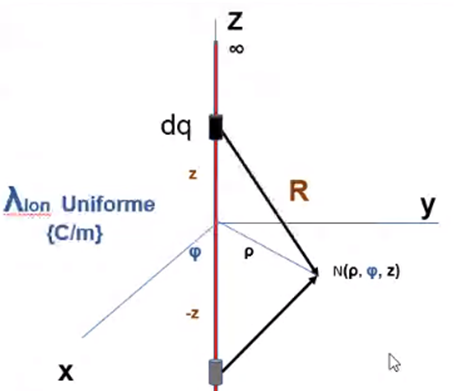
\includegraphics[width=.5\linewidth]{figures/longitudinal1.png}
\caption{Longitudinal distribution}
\label{longitudinal1}
\end{figure}

The Figure \ref{longitudinal2} show us a way to find the total electric field. 

\begin{figure}[H]
\centering
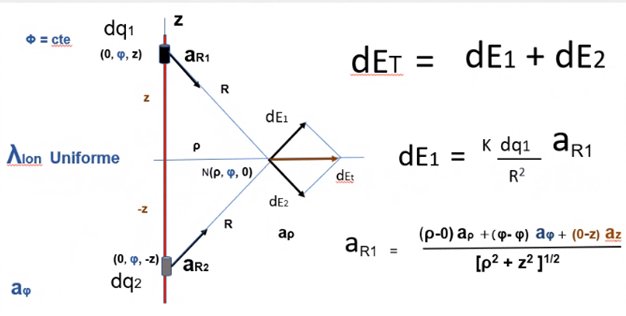
\includegraphics[width=.5\linewidth]{figures/longitudinal2.png}
\caption{Longitudinal distribution with symmetry}
\label{longitudinal2}
\end{figure}

We have the follow Equations
\begin{align*}
dE_T=dE_1+dE_2
\end{align*}

\begin{align*}
dE_1&=\frac{Kdq_1}{R_1^2}a_{R1}\\
a_{R1}&=\frac{(\rho -0)a_{\rho }+(\phi -\phi)a_{\phi }+(0-z)a_z }{\sqrt{\rho ^2 + z^2}}\\
dE_1&=\frac{Kdq_1}{(\rho ^2 + z^2)^{\frac{3}{2}}} (\rho a_{\rho }-za_z) 
\end{align*}

\begin{align*} 
dE_2&=\frac{Kdq_2}{R_2^2}a_{R2}\\
a_{R2}&=\frac{(\rho -0)a_{\rho }+(\phi -\phi)a_{\phi }+(0-(-z))a_z }{\sqrt{\rho ^2 + z^2}}\\
dE_2&=\frac{Kdq_2}{(\rho ^2 + z^2)^{\frac{3}{2}}} (\rho a_{\rho }+za_z) 
\end{align*}

The value of $E_T$ is:

\begin{align}
E_T&=\int_{-\infty }^{\infty } \frac{ k\lambda _L \rho dz}{(\rho ^2 + z^2)^{\frac{3}{2}}}a_{\rho }=k\lambda _L \rho \int_{-\infty }^{\infty } \frac{ dz}{(\rho ^2 + z^2)^{\frac{3}{2}}}a_{\rho } \\
\intertext{Or}
E_T&=\int_{0 }^{\infty } \frac{2 k\lambda _L \rho dz}{(\rho ^2 + z^2)^{\frac{3}{2}}}a_{\rho }=2k\lambda _L \rho \int_{0}^{\infty } \frac{ dz}{(\rho ^2 + z^2)^{\frac{3}{2}}}a_{\rho } \\
\intertext{And Finally}
E_T&=\frac{\lambda _L a_{\rho }}{2\pi \epsilon _0 \rho }  
\end{align}

\chapter{Modeling}

\begin{table}[H]
        \caption{The equivalent components of circuits}
        \label{DSA}
        \begin{center}
        \begin{tabular}{|c||c|}
        \hline        
         \textcolor{blue}{Capacitance}  &\textcolor{green}{Resistance}   \\ \hline
         $C=\frac{Q_e}{V}=\frac{\int D \cdot ds}{-\int E \cdot dL}  $  
         & $R=\frac{V}{I} = \frac{- \int E \cdot dL}{\int j \cdot dS}$  \\ \hline
         \textcolor{blue}{Inductance}& \textcolor{green}{Conductance} \\ \hline
        $L=\frac{\phi _{mag}}{I}=\frac{\int B \cdot dS}{\oint H\cdot dL}  $  
         & $G=\frac{I}{V}=\frac{\int j\cdot dS}{-\int E\cdot dL}$  \\ \hline
        \end{tabular}
        \end{center}
    \end{table}
    \vspace{0.2 cm}
    Comments
    
    \begin{itemize}
    \item $V=\int j \cdot ds$: Gauss's law for the current.
    \item $V=-\int E \cdot dL$: Negative sign is because a external force do the work.
    \item  $I=\oint H\cdot dL$: If you see the Maxwell equations, you can note that here be missing a term. According to the teacher, it is because only import the magnetic field. 

    
   
    \end{itemize}

    
\chapter{Efecto de los campos en los materiales}    

\begin{question}
¿Por qué se dañan los componentes eléctricos o electrónicos comúnmente?\\
Por el desgaste de los aislantes. Por ejemplo, un transformador se daña porque se hace un corto circuito al desgastarsen los aislantes.
\end{question}  

\begin{question}
¿Cuando un aislante cambia sus propiedades?\\
Ocurre cuando sus cargas ligadas se convierten en cargas libres. En un aislante hay pocas cargas libres.
\end{question}  
   
\section{Polarización}

El potencial se un dipolo en un punto N se puede plantear como:


\begin{figure}[H]
\centering
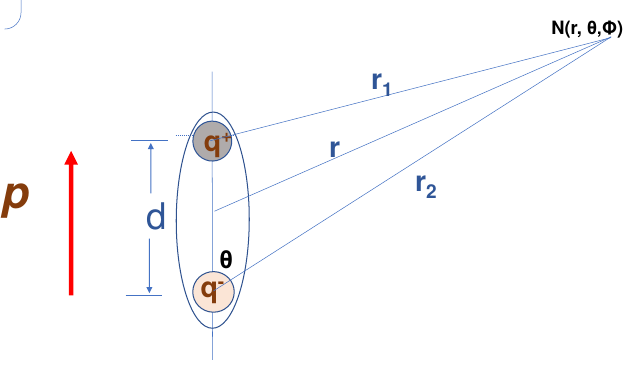
\includegraphics[width=.5\linewidth]{figures/pol1.png}
\caption{}
\label{pol1}
\end{figure}
\vspace{0.2cm}

El resultado es:


\begin{figure}[H]
\centering
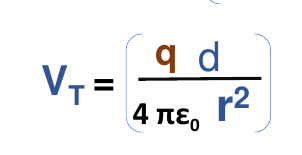
\includegraphics[width=.5\linewidth]{figures/pol2.png}
\caption{}
\label{pol2}
\end{figure}
\vspace{0.2cm}


El \textit{momento dipolar (p) } se define como

\begin{figure}[H]
\centering
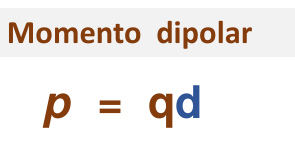
\includegraphics[width=.5\linewidth]{figures/pol3.png}
\caption{}
\label{pol3}
\end{figure}
\vspace{0.2cm}

Es la capacidad que tiene una carga en orientarse según el campo eléctrico. La \textit{(polarización P)} se puede plantear como:\\

Cuando no hay $\vec{E}$, las cargas están desorganizadas 
\begin{figure}[H]
\centering
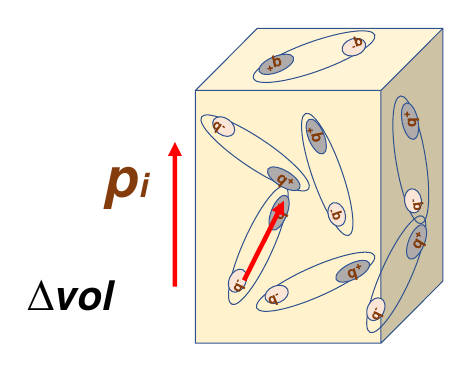
\includegraphics[width=.5\linewidth]{figures/pol5.png}
\caption{}
\label{pol5}
\end{figure}
\vspace{0.2cm}

En presencia de $\vec{E}$ Las cargas se organizan

\begin{figure}[H]
\centering
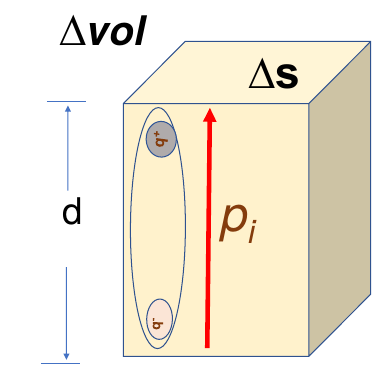
\includegraphics[width=.5\linewidth]{figures/pol51.png}
\caption{}
\label{pol51}
\end{figure}
\vspace{0.2cm}

Supongamos que hay una redistribución uniforme

\begin{figure}[H]
\centering
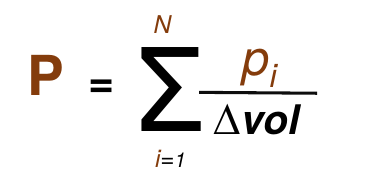
\includegraphics[width=.5\linewidth]{figures/pol4.png}
\caption{}
\label{pol4}
\end{figure}
\vspace{0.2cm}

\textit{P: La capacidad de generar polos por unidad de volumen}
\begin{sabias}
La polarización (P) en el vació es cero, porque allí no hay ningún material
\end{sabias}

\section{Carga Libre}



\begin{figure}[H]
\centering
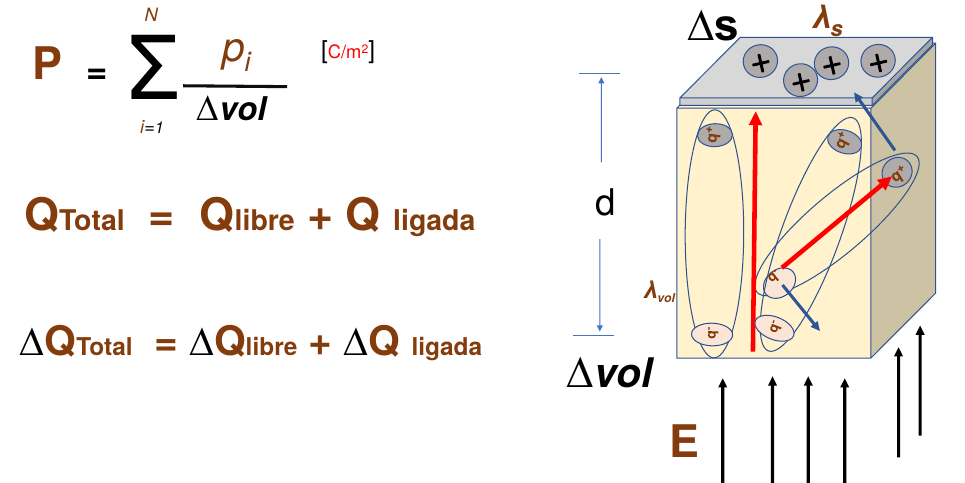
\includegraphics[width=1\linewidth]{figures/carFre.png}
\caption{}
\label{carFre}
\end{figure}
\vspace{0.2cm}

\begin{figure}[H]
\centering
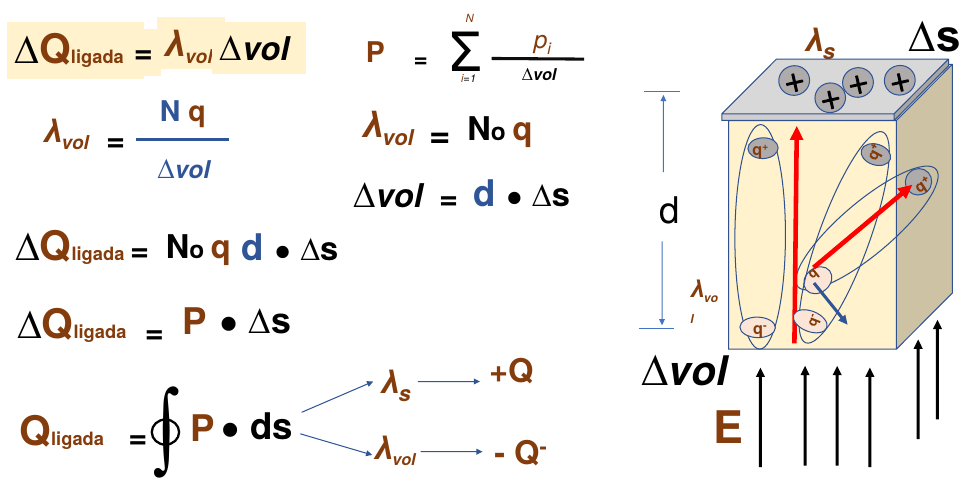
\includegraphics[width=1\linewidth]{figures/carFre2.png}
\caption{}
\label{carFre2}
\end{figure}
\vspace{0.2cm}

Para continuar con el procedimiento se elige la carga negativa, porque se quiere trabajar con diferenciales de volumen.

\begin{figure}[H]
\centering
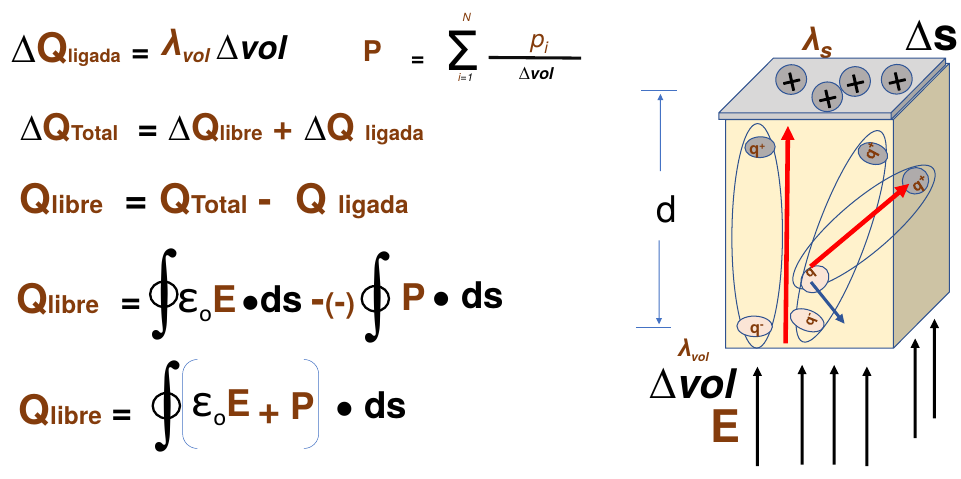
\includegraphics[width=1\linewidth]{figures/carFre3.png}
\caption{}
\label{carFre3}
\end{figure}
\vspace{0.2cm}

\begin{question}
¿Por qué se elige a $\epsilon _o$ para la carga total si estamos en un material?\\
Porque la mayor parte de la estructura se puede considerar vacío, por ejemplo en las estructuras cristalinas hay espacios intersticiales y en un núcleo atómico la mayor parte la compone el vacío.
\end{question}



\begin{figure}[H]
\centering
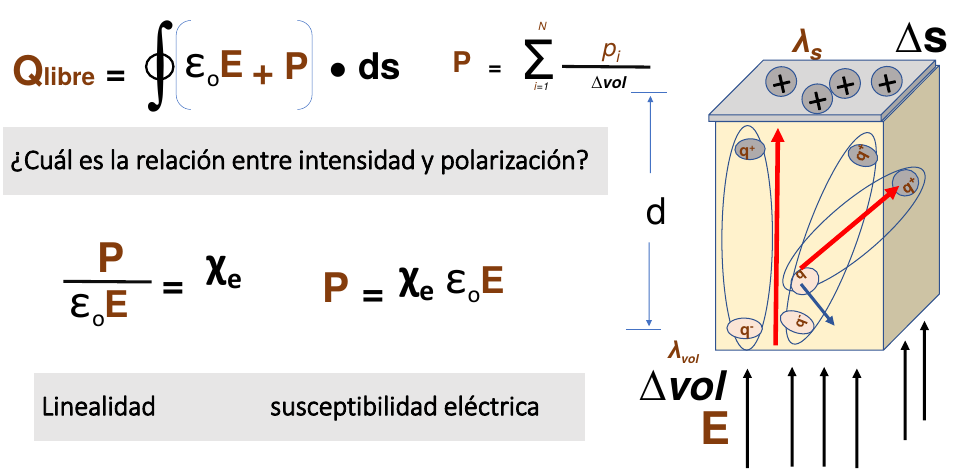
\includegraphics[width=1\linewidth]{figures/carFre4.png}
\caption{}
\label{carFre4}
\end{figure}
\vspace{0.2cm}

Donde
\begin{align*}
P: \text{Polarización}\\
\chi _e: \text{suceptividad eléctrica}\\
\epsilon _0: \text{Permitividad}
\end{align*}

En caso magnético \footnote{Es redundante decir Permeabilidad Magnética}
\begin{align*}
P: \text{Magnetización} \\
\chi _e: \text{Suceptividad Magnética}\\
\epsilon _0: \text{Permeabilidad } 
\end{align*}


\begin{figure}[H]
\centering
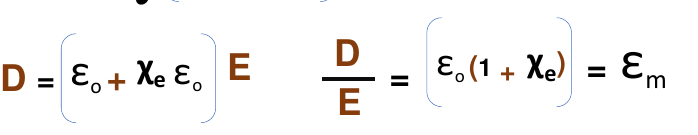
\includegraphics[width=1\linewidth]{figures/carFre5.png}
\caption{}
\label{carFre5}
\end{figure}
\vspace{0.2cm}


\begin{align*}
\epsilon _m \text{: Capacidad de producir flujo por unidad de area al aplicar una campo eléctrico}
\end{align*}

Además $\frac{\vec{D}}{\vec{E}}=\epsilon _0(1+\chi )$ si el campo es isotrópico, esto es que los vectores de densidad de campo eléctrico e intensidad estén en la misma dirección.



\begin{sabias}
En en el vacío $\chi =0$ porque no hay dipolos y $\epsilon _r=1$. En un material polar al aplicar $\vec{E}$ se polariza, en cambio en una dipolar  la nube aumenta al tener las mismas condiciones. 
\end{sabias}

Entonces en un materiar polar al aplicar un $\vec{E}$ se genera un campo secundario \textit{P} que refuerza a este primero.

\begin{figure}[H]
\centering
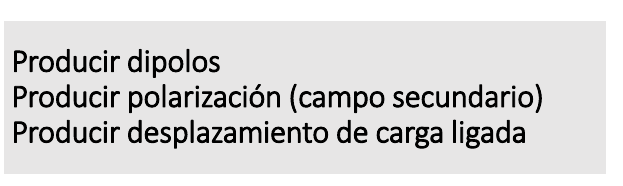
\includegraphics[width=1\linewidth]{figures/carFre6.png}
\caption{}
\label{carFre6}
\end{figure}
\vspace{0.2cm}


\section{Disrupsión}
De $E_0-E_2$: linealidad, de $E_2-E_{c}$ : Ionización (punto antes de la disrupción) y de $E_{c}-$: Disrupción
\begin{figure}[H]
\centering
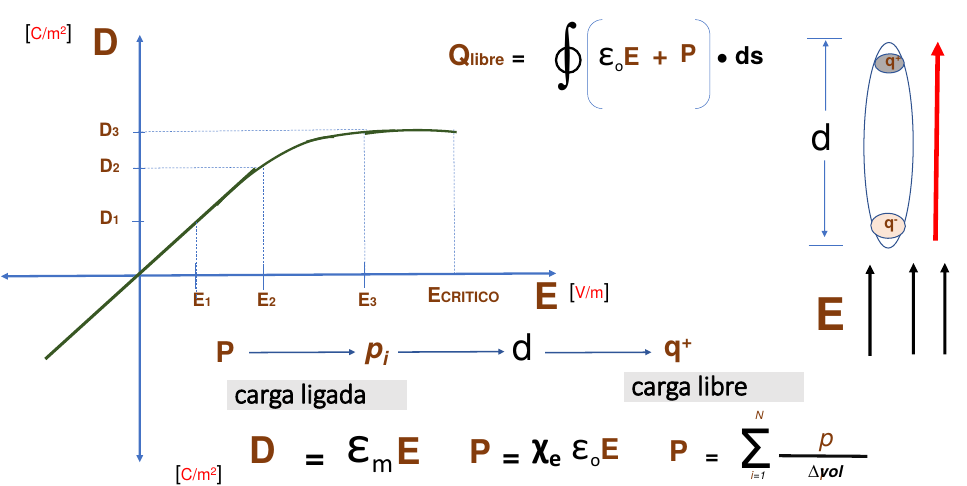
\includegraphics[width=1\linewidth]{figures/dis.png}
\caption{}
\label{}
\end{figure}
\vspace{0.2cm}

\begin{definition}[Disrupción]

\end{definition}


\begin{exercise}[Caucho]
Imagine que estire un caucho, algunas moléculas se van estirando hasta que en algún momento su se aplican más fuerza este se va a romper. Algo curioso es que cuando se deja de estirar queda en algunas ocasiones deformado de por vida.
\end{exercise}

Por ello, hay que tener cuidado con las $\vec{E}$ que se le aplican a un material porque al llevar a los extremos se corre con el peligro de no poder mantener las características iniciales.

\begin{figure}[H]
\centering
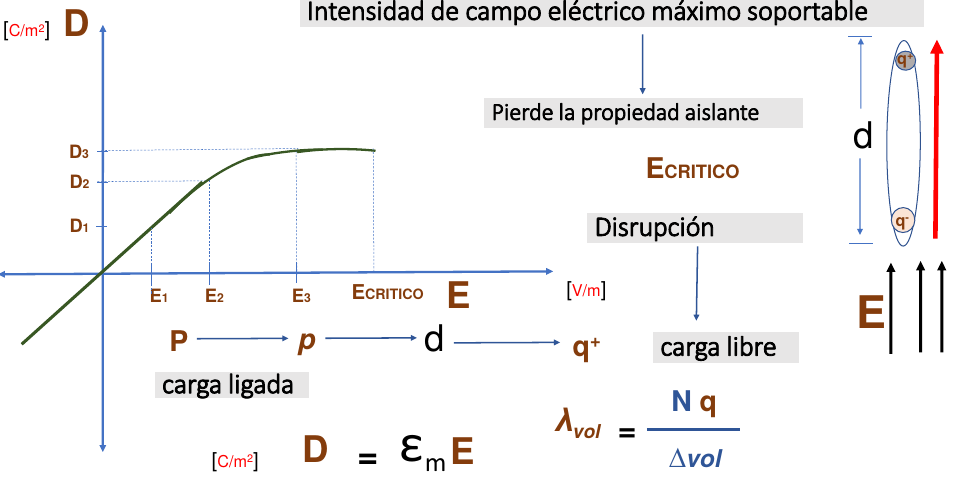
\includegraphics[width=1\linewidth]{figures/dis1.png}
\caption{}
\label{}
\end{figure}
\vspace{0.2cm}

\begin{figure}[H]
\centering
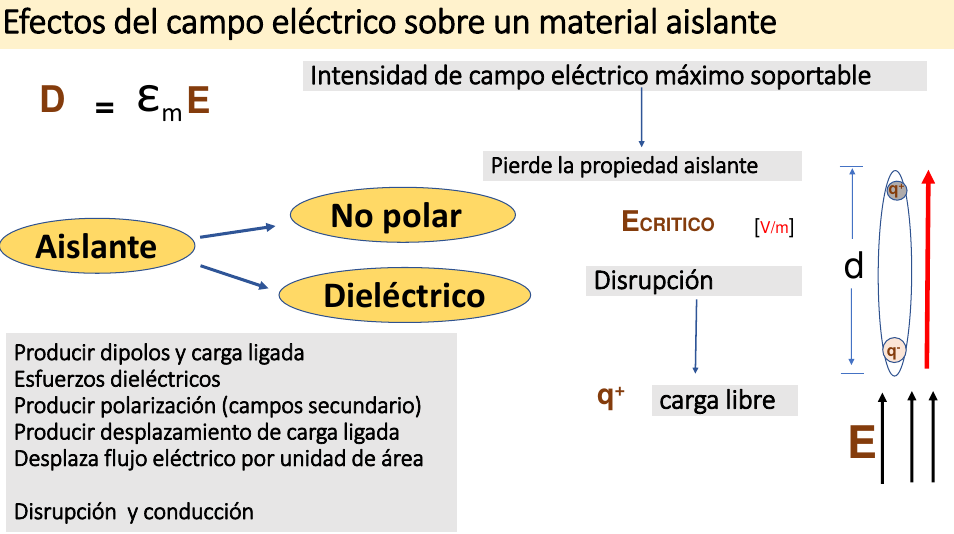
\includegraphics[width=1\linewidth]{figures/dis2.png}
\caption{}
\label{}
\end{figure}
\vspace{0.2cm}

\begin{question}
¿Cuál es la diferencia conceptual entre ionización y rigidez dieléctrica?\\
La rigidez dieléctrica es el máximo $\vec{E}$ en el cual el material pierde su capacidad de aislante y pasa a ser conductor. Por otra parte, la Ionización...
\end{question}

\section{Cálculo de trabajo}

\textcolor{blue}{Anexar presentaciones y hojas 2020-06-08 s1 y s2}
\begin{itemize}
\item La energía en una linea de transmisión está en todo el espacio, no solo en el conductor.
\item $\frac{ \vec{D}}{ \vec{E}}=\epsilon _m$ caracteriza el medio.
\item $\frac{\Delta W_T}{\Delta _{vol}}$ se denomina densidad volumétrica de energía y expresa la cantidad de de energía que se puede almacenar por unidad de volumen a partir de un $\vec{E}$ aplicado.
\item $\epsilon_m=\frac{ \vec{D}}{\vec{E}}$ La capacidad de un material para generar flujo de intensidad por unidad de área en función de una intensidad aplicada. Note que las unidades son $\left[ \frac{F}{m} \right]=\left[ \frac{c/m^2}{\text{ \textcolor{red}{$v/m$}} }\right]$ el término en rojo significa que que es acción a distancia. 
\end{itemize}

La densidad volumétrica de energía tiene la similitud con la carga energía de un capacitor:
\begin{equation}
dw=vdq \Rightarrow W=\int Vdq \Rightarrow \int \frac{q}{C} dq \Rightarrow \frac{q^2}{2C}=\frac{cv^2}{2}
\end{equation}

\begin{itemize}
\item Similitud entre dividir y oponerse.
\item Similitud entre el producto punto y la capacidad para almacenar energía.
\end{itemize}

\begin{question}
¿Qué técnica propone para protegernos del campo eléctrico?\\
\begin{itemize}
\item Distanciamiento
\item Hacer que las concentraciones disminuyan
\end{itemize}
\end{question}

\begin{question}
¿Qué significa para usted 100 $\frac{v}{m}$?\\
La $\vec{E}$ de la atmósfera ronda entre 100-150 $v/m$. En momentos anteriores a una tormenta, este valor pude ser 10 o 100 veces mayor. 
\end{question}

\begin{question}
¿Cuál es la intensidad de campo eléctrico en la toma de la casa?\\
Si suponemos que hay 1cm de distancia entre la fase y el neutro, se pude decir que la intensidad de campo eléctrico es $\frac{120 Vrms}{1cm}$. Esa intensidad dada en $\frac{12000 Vrms}{m}$ estaría correcta pero usted no va a observar una distancia de 1m de la fase al neutro. Otra manera incorrecta de dar ciertas magnitudes es la potencia de un rayo en $KVh$ porque el rayo nunca va a durar una hora, este solo se presenta en cuestión de milisegundos. Los promedios tienden a perder parte de la información, por ejemplo si Esteban y Sebastian se están en una casa y algunos de ellos se come los diez sándwiches que habían, alguien puede decir que en promedio se comieron 5 lo que es verdad según el significado de promedio, pero no se acerca a la realidad.
\end{question}


\begin{sabias}
En en ecuador el 99\% de las tormentas son con lluvia. En cambio, cerca a los polos suceden tormentas.
\end{sabias}

 \begin{question}
 ¿Qué le pasó al transbordador para que no pudiera despegar?\\
 Cuenta con dispositivos que medían constantemente la $\vec{E}$ y no cumplió con las especificaciones adecuadas. Además, debido a que el tanque tiene Nitrógeno y Oxígeno era peligrosa alguna explosión.
 \end{question}

 \begin{question}
 ¿Puedo almacenar la energía de un rayo?\\
 Un rayo tiene mucha potencia, pero poca energía.
 \end{question}


 \begin{question}
 ¿Por qué $\epsilon _r$ del aire es similar a la del vacío?\\
 Porque las moléculas no se polarizan, el campo eléctrico en el aire hace la que las moléculas se muevan a una velocidad impresionante pero no logra la polarización y por lo tanto $ \chi \approx 0$
 \end{question}


 \begin{exercise}
 ¿Para que me sirven una densidad de energía de $4.225 \mu \frac{J}{m^3}$ ?\\
 \end{exercise}


\bibliography{myBooks}
\bibliographystyle{unsrt}

\end{document}
